% Copyright (C) 2014-2024 by Thomas Auzinger <thomas@auzinger.name>

\documentclass[draft,final]{vutinfth} % Remove option 'final' to obtain debug information.

% Define convenience functions to use the author name and the thesis title in the PDF document properties.
\newcommand{\authorname}{Alexander Rinsche} % The author name without titles.
\newcommand{\thesistitle}{Context-sensitive Semantic Search in Graphs} % The title of the thesis. The English version should be used, if it exists.

% Create the XMP metadata file for the creation of PDF/A compatible documents.
\begin{filecontents*}[overwrite]{\jobname.xmpdata}
\Author{\authorname}                                    % The author's name in the document properties.
\Title{\thesistitle}                                    % The document's title in the document properties.
\Language{de-AT}                                        % The document's language in the document properties. Select 'en-US', 'en-GB', or 'de-AT'.
\Keywords{a\sep list\sep of\sep keywords}               % The document's keywords in the document properties (separated by '\sep ').
\Publisher{TU Wien}                                     % The document's publisher in the document properties.
\Subject{Thesis}                                        % The document's subject in the document properties.
\end{filecontents*}

% Load packages to allow in- and output of non-ASCII characters.
\usepackage{lmodern}        % Use an extension of the original Computer Modern font to minimize the use of bitmapped letters.
\usepackage[T1]{fontenc}    % Determines font encoding of the output. Font packages have to be included before this line.
\usepackage[utf8]{inputenc} % Determines encoding of the input. All input files have to use UTF8 encoding.

% Extended LaTeX functionality is enables by including packages with \usepackage{...}.
\usepackage{amsmath}    % Extended typesetting of mathematical expression.
\usepackage{amssymb}    % Provides a multitude of mathematical symbols.
\usepackage{mathtools}  % Further extensions of mathematical typesetting.
\usepackage{microtype}  % Small-scale typographic enhancements.
\usepackage[inline]{enumitem} % User control over the layout of lists (itemize, enumerate, description).
\usepackage{multirow}   % Allows table elements to span several rows.
\usepackage{booktabs}   % Improves the typesetting of tables.
\usepackage{subcaption} % Allows the use of subfigures and enables their referencing.
\usepackage[ruled,linesnumbered,algochapter]{algorithm2e} % Enables the writing of pseudo code.
\usepackage[dvipsnames,table]{xcolor} % Allows the definition and use of colors. This package has to be included before tikz.
\usepackage{nag}        % Issues warnings when best practices in writing LaTeX documents are violated.
\usepackage{todonotes}  % Provides tooltip-like todo notes.
\usepackage{morewrites} % Increases the number of external files that can be used.
\usepackage[a-2b,mathxmp]{pdfx}      % Enables PDF/A compliance. Loads the package hyperref and has to be included second to last.
\usepackage[acronym,toc]{glossaries} % Enables the generation of glossaries and lists of acronyms. This package has to be included last.

% Set PDF document properties
\hypersetup{
    pdfpagelayout   = TwoPageRight,           % How the document is shown in PDF viewers (optional).
    linkbordercolor = {Melon},                % The color of the borders of boxes around hyperlinks (optional).
}

\setpnumwidth{2.5em}        % Avoid overfull hboxes in the table of contents (see memoir manual).
\setsecnumdepth{subsection} % Enumerate subsections.

\nonzeroparskip             % Create space between paragraphs (optional).
\setlength{\parindent}{0pt} % Remove paragraph indentation (optional).

\makeindex      % Use an optional index.
\makeglossaries % Use an optional glossary.
%\glstocfalse   % Remove the glossaries from the table of contents.

% Set persons with 4 arguments:
%  {title before name}{name}{title after name}{gender}
%  where both titles are optional (i.e. can be given as empty brackets {}).
\setauthor{}{\authorname}{}{male}
\setadvisor{Prof.}{Emanuel Sallinger}{}{male}

% For bachelor and master theses:
\setfirstassistant{Dr.}{Eleonora Laurenza}{}{female}
%\setsecondassistant{Pretitle}{Forename Surname}{Posttitle}{male}
%\setthirdassistant{Pretitle}{Forename Surname}{Posttitle}{male}

% For dissertations:
%\setfirstreviewer{Pretitle}{Forename Surname}{Posttitle}{male}
%\setsecondreviewer{Pretitle}{Forename Surname}{Posttitle}{male}

% For dissertations at the PhD School and optionally for dissertations:
\setsecondadvisor{Pretitle}{Forename Surname}{Posttitle}{male} % Comment to remove.

% Required data.
\setregnumber{12120519}
\setdate{01}{01}{2025} % Set date with 3 arguments: {day}{month}{year}.
\settitle{\thesistitle}{Kontext-sensitive Semantische Suche in Graphen} % Sets English and German version of the title (both can be English or German). If your title contains commas, enclose it with additional curvy brackets (i.e., {{your title}}) or define it as a macro as done with \thesistitle.
\setsubtitle{Optional Subtitle of the Thesis}{Optionaler Untertitel der Arbeit} % Sets English and German version of the subtitle (both can be English or German).

% Select the thesis type: bachelor / master / doctor.
% Bachelor:
\setthesis{bachelor}
%
% Master:
%\setthesis{master}
%\setmasterdegree{dipl.} % dipl. / rer.nat. / rer.soc.oec. / master
%
% Doctor:
%\setthesis{doctor}
%\setdoctordegree{rer.soc.oec.}% rer.nat. / techn. / rer.soc.oec.

% For bachelor and master:
\setcurriculum{Software \& Information Engineering}{Software \& Information Engineering} % Sets the English and German name of the curriculum.

% Optional reviewer data:
\setfirstreviewerdata{Affiliation, Country}
\setsecondreviewerdata{Affiliation, Country}


\begin{document}

\frontmatter % Switches to roman numbering.
% The structure of the thesis has to conform to the guidelines at
%  https://informatics.tuwien.ac.at/study-services

\addtitlepage{naustrian} % German title page.
\addtitlepage{english} % English title page.
\addstatementpage

\begin{danksagung*}
\todo{Ihr Text hier.}
\end{danksagung*}

\begin{acknowledgements*}
\todo{Enter your text here.}
\end{acknowledgements*}

\begin{kurzfassung}
\todo{Ihr Text hier.}
\end{kurzfassung}

\begin{abstract}
Semantic Search is the concept where a search over document corpus does not look for traditional word or partial word matches, but instead considers the embeddings of the query and the corpus to be searched encoded by some model. Performing a search then equates to calculating some distance metric such as euclidian distance, cosine similarity, etc. between the query embedding and all respective documents. This results in a total ordering of all documents by how similar the model evaluates the contents to the posed query. Clearly, this necessitates the model to have a decent understanding of the domain and for synonimic or otherwise related terms to achieve higher similarity scores, finetuning appears paramount, especially in corporate and technical environments with specialized langugage and vocabulary. An attempt to alleviate or at least lessen this issue will be proposed. Additionally, a semi-supervised learning pipeline to easily iterate over attempts will be proposed. Finally, a proper architecture to encapsulate this pipeline in a production-ready search engine that is easily (re-)deployable to a kubernetes cluster and can scale with demands with the necessary things in place to migrate the pipeline to an online reinforcement learning system in future work.
\end{abstract}

% Select the language of the thesis, e.g., english or naustrian.
\selectlanguage{english}

% Add a table of contents (toc).
\tableofcontents % Starred version, i.e., \tableofcontents*, removes the self-entry.

% Switch to arabic numbering and start the enumeration of chapters in the table of content.
\mainmatter

\chapter{Introduction}

What is the definition of Information? To further specify the question, such a definition should cover the following commonly observed properties of information:
\begin{itemize}
    \item The same sentence contains a different amount of information depending on the receiver and their context
    \item It's verb ''to inform'' means to convey a fact that should influence someone's behavior.
    \item An ''informed decision'' means to be aware of as many relevant facts as possible concerning a certain decision.
\end{itemize} 
By those properties, the definition of information for this thesis will be ''facts or knowledge relevant to a receiver that influence their behavior or decisions''. The amount of information can be determined by the severity of change in their actions depending on getting or missing a said piece of information. For a machine learning model, this can essentially be measured by loss. A data sample with a high loss obviously contains more information than the last ten data samples that the model predicted correctly and therefore had little to no loss. 

From this there is a clear distinction between a Knowledge Base and a Information System: While a Knowledge Base is a collection of facts or, more generally speaking, knowledge, an Information System needs to actively filter the facts relevant to a user or a query. 
%So although a database can be considered a perfectly suitable Information System to experienced developers, for a common user there is too much (to them) uninteresting information and overhead attached to properly use it. 
For a Knowledge Base to become an Information System, a mechanism that produces the relevant information to their users at the moment where it becomes relevant, without additional overhead of filtering out unnecessary data, is paramount. In this thesis we will explore and evaluate one possible mechanism leveraging Text Embeddings and Knowledge Graph Technology.

\section{Motivation}
The recent success of transformer architectures has affected most areas of Computer Science to some degree. In the field of Information Retrieval and Search through document corpi, the technique of Semantic Search has gained new traction. While previous approaches like one hot encodings or continuous bag of words all had their shortcomings, new transformer architectures are able to capture complex relationships and meanings of words in dense vectors and through the attention mechanism that the transformer architectures all share even ambiguities of words are representable in these models.
The price is the high initial cost to train these models, the billions of parameters that need to be loaded in active memory and additional finetuning that is often required when it comes to more specialized domains.
The computational resources required for these tasks are still infeasible to most individuals and even many companies, which is why big tech companies like Google and OpenAI are currently so successful. The aim of this thesis is to propose an alternative architecture where semantic embeddings do not have to be perfect but can be improved later on without fine-tuning of the embedding model itself and rather through exploiting additional information about the domain. The proposed approach should also produce a decent semantic search and maybe even a recommendation system that can take user-based relevance into account. For this to be possible, the input data needs to be more than just a loose collection of documents, but a set of documents and users organized and linked in a rich taxonomy. By leveraging the information encoded in a neighborhood in such a graph, additional information about the context should be includable through graph based learning methods such as Graph Neural Networks (GNNs).


\section{Data Sources}
The necessary data for training and evaluating the model was obtained from qibri.
qibri is a Knowhow Management System targeted at medium to large companies with highly specialized domain-specific knowledge. Its purpose is to manage and unify all documentation of Knowhow in a central place, to create a better overview of how well the core processes and products are documented and provide the necessary documentation to an employee when they needed. It has several mechanisms to encourage users to regularly check and update the Knowhow that they are responsible for, a versioning and approval process system to make sure changes are transparent, can be backtracked and are formally accepted by decision makers. Knowledge retrieval is particularly difficult in this context, however - there's a lot of information that might seem relevant when searching for a specific subject, but usually a lot of it just is not relevant to the user who started the search. So, although a document might seem to contain a lot of keywords relevant to a given search, it might still be the case that it just is not relevant due to it's particular scope and target audience within a company. To mitigate this, all documents and users are organized in a taxonomy, containing locations, departments, relevant topics, etc. Using this taxonomy, one can quickly get an idea which documents are more closely related to a user's daily work and which might be less relevant, just by using the distances between them. Unifying a semantic search with the relevance scoring particular to the user triggering the search will be another area of exploration of this thesis, although the necessary data to evaluate such a joint search is currently not available and will only be obtainable through a feedback loop.

\section{Problem Statement}
Finding, optimizing and verifying such a system unfortunately exceeded the scope of a bachelor thesis. Therefore, the focus of this work will be on creating a sensible framework for quickly iterating over different versions. The main challenges this thesis posed were
\begin{description}
    \item[history preservation] i.e. incorporating some kind of versioning so that different extraction runs can easily be compared to each other.
    \item[extendability] building the pipeline in a way such that changes to the data extraction and the embedding process are ''easy'' to implement.
    \item[ease of deployment] - due to the classic difficulties of evaluating a recommender system or a search engine (difficulties defining ''correct'' results, relevances for different people, etc.), one of the main requirements imposed by qibri was the option to quickly deploy to production and to test it there.
\end{description}
In addition to that, there are three iterations of the system that are going to be explicitly compared: A naive Semantic Search, A static Message Passing Contextualization, where no parameters are actually learned and context is statically aggregated and a proper GNN-based approach, where actual learnable parameters are fit. These steps should give a decent first idea if the proposed methodology seems promising or not.

An additional necessity that was posed by qibri was the option for logical filtering. The prior search engine, which was purely based on boolean logical filters and classical full text search, provided the user the option to filter out results based on simple logical filters such as linked taxonomies, authors and other simple true/false filters.

\chapter{Sentence Embeddings}
This section will focus on establishing the necessary terminology and background information necessary to understand the Machine Learning and AI aspects of this thesis. Firstly, a brief overview over methods to represent text as a low-dimensional vector will be provided. 
\section{Word2Vec}
Representing words or, more generally speaking, text, as (relatively) low-dimensional embedding vectors (instead of the trivial method of one-hot-encoding a dictionary) such that relative distances and orientation capture some notion of meaning is one of if not the main topic of Natural Language Processing (NLP). One of the first big successes on this field was Word2Vec, which was published in a paper by Mikolov et al., at Google, in 2013. This technique uses a sliding window approach where every word in the vocabulary of the model gets projected to a dense vector and these vectors are then fit using one of two methods: \textit{Continuous bag of words} or \textit{continuous skip-gram}. Both of these methods use simple linear transformations where the one-hot-encoded word vector gets projected to a dense vector space with dimensionality $\mathcal{D}$, while the bag-of-words approach uses the surrounding to predict a missing word, the skip-gram version uses a specific input word to predict the surrounding. Figure \ref{fig:word2vec} shows a comparison between these learning approaches.
\begin{figure}
    \centering
    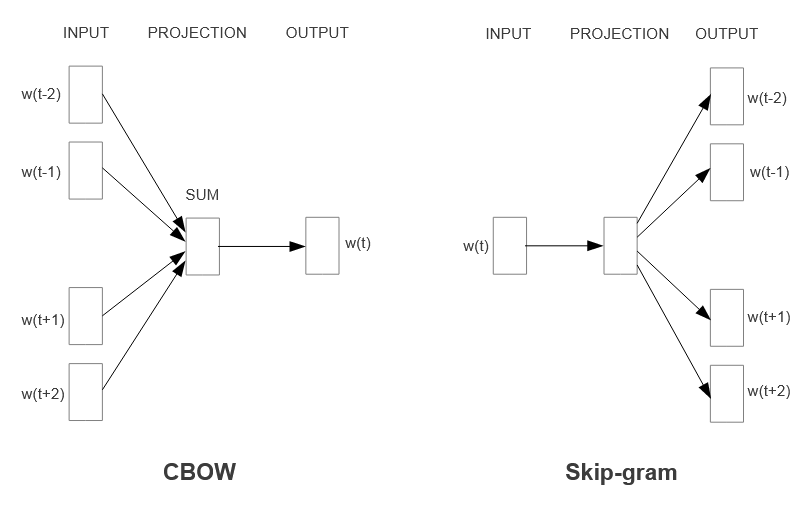
\includegraphics[width=0.9\linewidth]{thesis-figures/word2vec.png}
    \caption{Contrasting the CBOW and Skip-gram word2vec approach \cite[p. 5]{word2vec_preprint}}
    \label{fig:word2vec}
\end{figure}
The novel part of these approaches is that the predicitons are computed by another simple linear layer followed by a softmax, without any non-linearities or any larger depth. \cite{word2vec_preprint} This however suffices to learn relationships like $v('France') - v('Paris') + v('Madrid') \approx v('Spain')$, while still being quite efficient to compute. \cite{word2vec_official} The limitations arise from more complex relationships and a deeper understanding of text. By construction, Word2Vec has no mechanism to alter meaning by context, it does not even capture the sequence of words. As the term "Bag of Words" implies, the model considers no notion of ordering, words that appear before and after are summed up, averaged, and then the most similar word is predicted. The skip-gram approach also only predicts words that are also likely to appear given a specific input word, not the \textit{next} or \textit{previous} words. In addition to that, words that have several different meanings like ''bear'' or ''bow'' also are not distinguished. The semantic nuances are accumulated in a single embedding vector and any predictions are ambiguous if they were a result of the verb or the noun. A final drawback is that words that were not included in the initial vocabulary can't be assigned an embedding later on, word2vec can't assign new embeddings on the fly. With these strengths and drawbacks in mind, let's consider a more recent alternative. 


\section{The Transformer Architecture}
The paper \textit{Attention is all you need} \cite{vaswani_attention_2017} by Vaswani et al. first describes the Transformer architecture, now prominent in Large Language Models. In contrast to Word2Vec, embeddings in this architecture consist of the vector associated with the token according to the vocabulary plus a positional encoding (a combination of sine and cosine functions depending distinct for every dimension of the embedding). Additionally, although the training process bears some resemblance to the CBOW variant of Word2Vec, there are some major improvements. Instead of just predicting \textbf{a} word in a sentence based on an unordered bag consisting of previous and following words, the training process used a sequence of words as an input and the task was to predict the next word. The ''byproduct'' of this process is essentially one of the earlier versions of ChatGPT - a model that predicts what the next word (or rather token, which might also be something like a syllable) should be in a conversation repeatedly. The internal architecture to make predictions differs heavily from the initial Word2Vec model. Several components are stacked in parallel and sequentially to ensure that each word embedding incorporates the context of all of it's neighborhood (or only its predecessors, depending on the mask used). From a birds's eye view you can separate the transformer into two parts: The encoder and the decder. The encoder takes the initial input text, passes it through its network, and then passes it on to the decoder. Depending on training or inference time, the decoder either gets the target text or the generated response up until this point as an input, passes it through it's first layers, merges it together with the data received from the encoder, passes the result through the following layers and uses that to assign probabilities to all possible output-tokens to indicate their likelihood of being the next in the sequence. Figure \ref{fig:transformer-architecture} was taken from the paper by Vaswani et al. and provides a good overview of the transformer's architecture. 
\begin{figure}
    \centering
    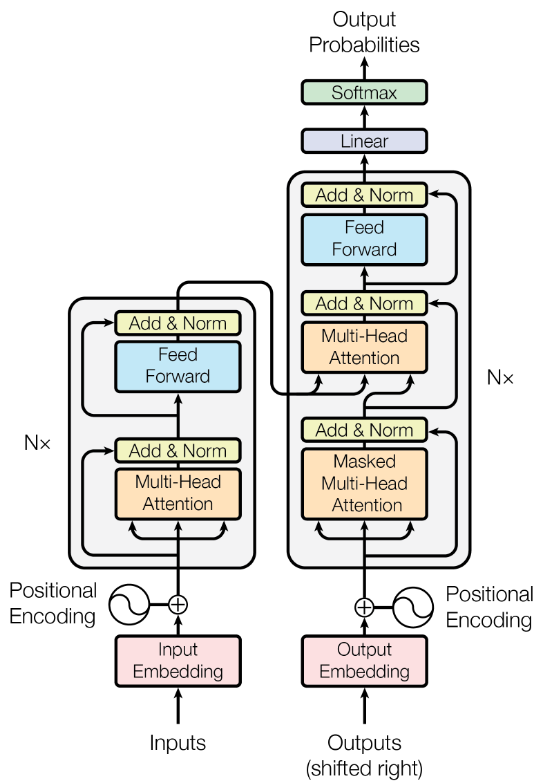
\includegraphics[width=0.5\linewidth]{thesis-figures/Transformer-Architecture.png}
    \caption{The architecture of the transformer model \cite[p. 3]{vaswani_attention_2017}}
    \label{fig:transformer-architecture}
\end{figure}As clearly illustrated by the diagram, both blocks each consist of multiple layers, the most important part, which will be briefly explained, are the \textit{self-attention}/\textit{multi-head-attention} layers. Self-attention lies of the core of incorporating the context and, as the paper title suggests, is all you need. Attention functions consist of a query and a set of key-value pairs as input, and their output is a weighted sum of the values biased by some compatibility function applied to the query and the corresponding key. This particular type of attention corresponds to this function: 
$$\mathbf{Attention}(Q,K,V) = softmax(\frac{Q \cdot K^T}{\sqrt{d_k}}) \cdot V$$
In a scenario where all of these are vectors or rather embeddings, it has an additional benefit of being easily parallelizable by using matrices instead, thereby enabling highly efficient GPU computations.\\
Self-attention is used in several different parts of a transformer. In the encoder block, it is used so that a singular word (or token) embedding incorporates the context of surrounding words and semantic connections become present. The paper even states that it appears to be benefitial to use several Self-attention layers in parallel, concatenating the results and applying a linear transformation, which suggests that there are several distinct levels of semantics that connect different parts of a text corpus (that are learned). This is called multi-head attention. Figure \ref{fig:paying-attention} shows a graphic illustration of both attention mechanisms
\begin{figure}
    \centering
    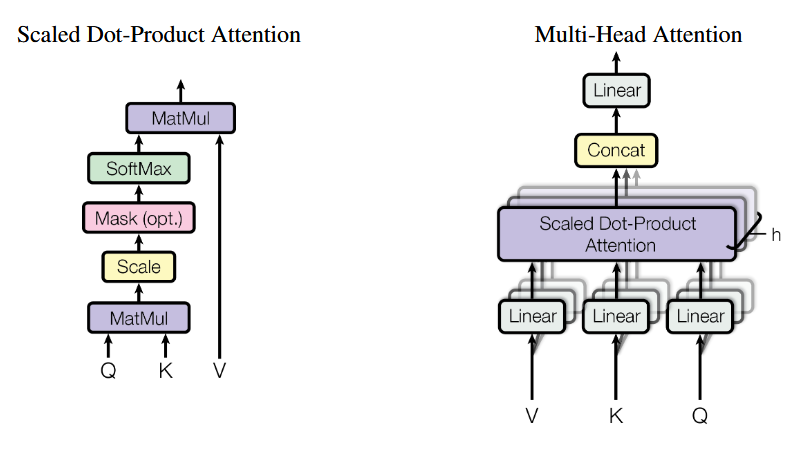
\includegraphics[width=1.0\linewidth]{thesis-figures/Attention.png}
    \caption{Self-attention (left) and Multi-Head Attention (right) \cite[p. 4]{vaswani_attention_2017}}
    \label{fig:paying-attention}
\end{figure}
The next use in the architecture is in the first layers of the decoder stack. The idea is the same as in the encoder, however, every word embedding is only allowed to use its \textbf{predecessors} as context, following embeddings are masked out. This is to ensure that the model learns to predict the next word in the output and does not use information present only in the training as an unwanted shortcut. The final use of an attention layer lies in the mergeing of encoder and decoder stacks. In this case  the question posed is ''Which parts of the input are related to which parts of the output''. Or, in terms of the paper ''This allows every position in the decoder to attend over all positions in the input sequence.'' \cite[p. 5]{vaswani_attention_2017}

\section{Generalizing Transformers}
The final step in the ladder regarding Text embeddings that will be briefly explained, is BERT, which stands for Bidirectional Encoder Representations from Transformers. While the initial transformers purpose was purely generative in nature, BERT is more a jack-of-all-trades type of model. It's used for tasks such as question answering where it finds the answer to a question within a given paragraph, sentiment analysis, classifying inferences between two sentences, semantic similarities and many more. There are several new concepts it introduced: Fully bidirectional attention mechanisms without masking - while the initial Transformer architecture by Vaswani et al. suggested Masking in the self-attention layers to prevent ''cheating'', BERT only uses masks in the actual training data, there is no masking in the entire architecture. This enables word embeddings to attend to the entire context, not only predecessors or successors. The way this is achieved is by altering the (pre-)training task - instead of predicting the next token, parts of the input are randomly masked and the task of the model is to predict the initial token which was supposed to be there. Additionally, the paper demonstrated how a single pretrained BERT instance can easily be finetuned to several different tasks - and outperformed many task-specific architectures at the time. The general architecture is identical to the encoder stack of the initial transformer architecture discussed previously. An input can be a single piece of text, or two connected halves, which are tokenized by a vocabulary that is built up of likelihood-based word and subword fragments with WordPiece \cite{wu_googles_2016} and then fed through the neural network. A special addition is a starting token ($\mathtt{[CLS]}$), which is prepended to each statement. This can then used for classification tasks later on. The $\mathtt{[SEP]}$ token is used to split the input into two segments, for tasks like quesion answer pairs and sentence inference. 
\begin{figure}[h!]
    \centering
    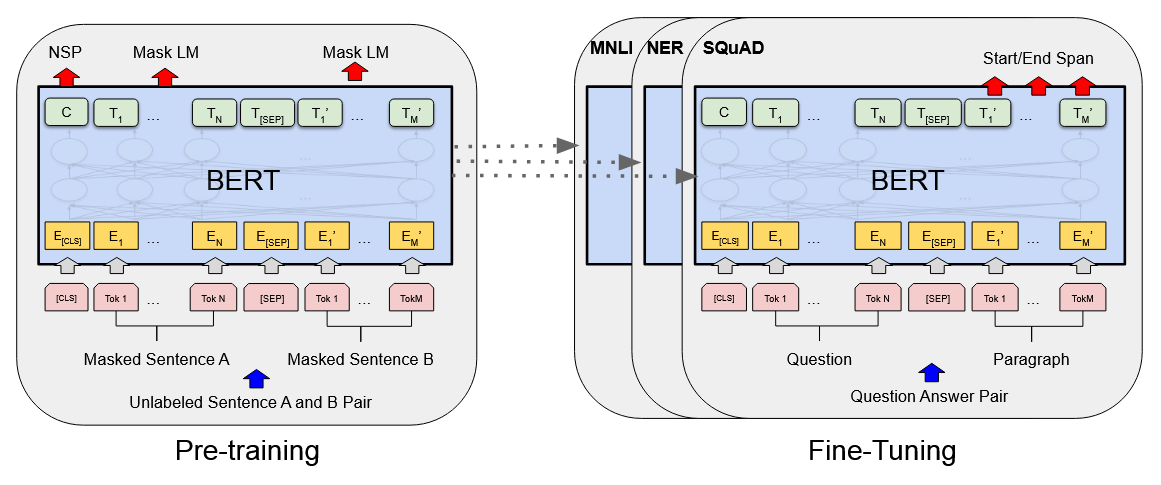
\includegraphics[width=0.9\linewidth]{thesis-figures/BERT-Architecture.png}
    \caption{Overview over the training process of a BERT model. \cite[p. 4173]{BERT}}
    \label{fig:BERT-training-setup}
\end{figure}
Figure \ref{fig:BERT-training-setup} illustrates the training process with a single pre-training and any arbitrary amount of fine-tuning for task specific heads. The output of the neural network is a set of text embeddings for each token of the input with context information from all other tokens. These are what can then be used for the previously mentioned downstream tasks. The pre-training consists of the aforementioned masking, dubbed ''Masked Language Model'' or MLM for short, and Next Sentence Prediction (NSP). For NSP, the model gets two sentences and has to predict if the second one follows the first in the original text corpus, or if it is a non-connected random sentence. For this task, the embedding of the $\mathtt{[CLS]}$ token at the beginning of the sequence is used. \cite{BERT}

\chapter{Graphs in Machine Learning}
\section{Knowledge Graphs}
A Knowledge Graph (KG) can formally be described as a set of triples of the form 
$\mathtt{< head,\ relation,\ tail>}$. The ''Knowledge'' part from a Knowledge Graph is that each part of a triple is supposed to reference some sort of real-world entity or concept. Therefore each reference has some sort notion of semantics with additional \textit{Knowledge} attached, which can be explicitly or implicitly modeled in the Knowledge Graph. Instances of Knowledge Graphs include (but are not limited to) the financial domain \cite{Bellomarini_Magnanimi_Nissl_Sallinger_2021}, where ownership, trade and similar relations form the links between people, companies or even entire countries, the bio-medical domain \cite{Lu_Goi_Zhao_Wang_2025}, where molecular structures, proteins etc. are used to model interactions and likelihoods of diseases, toxins and other substances relevant to modern medicine, and many more.

There are several benefits from using Knowledge Graphs to model your domain. Firstly, the aforementioned data model is very simple and can be represented in all kinds of data stores (not limited to graph stores!). Additionally, it's a powerful abstraction that enables sophisticated reasoning over a simple interface while still being able to tap into all the underlying complexity at will. Finally, there are well-established methodologies from the fields of reasoning and inference as well as machine learning, which are easily applicable to KGs. From the reasoning/database disciplines, there are tools such as Datalog, Answer Set Programming and Ontology-based reasoning such as the Semantic Web Stack with OWL and RDF. As for machine learning, models such as Knowlege Graph Embeddings (KGEs) and Graph Neural Networks (GNNs) are prime examples. GNNs will be further discussed in the next section, as they are a key part of this thesis. KGEs are a model that tries to map a set of triples (and thereby a Knowledge Graph) in a vector domain, where the nodes (which are represented by the heads and tails of the triples) are represented as points in this domain and relations are some sort of operation or formula for a pair of nodes to determine if the model predicts there to be an edge between the two or not. A classic example from literature is TransE, where relations are simple offset vectors and an edge is predicted as true iff the following equation holds true: $$embed(\mathtt{head}) + embed(\mathtt{relation}) \approx embed(\mathtt{tail})$$ 

The reason why this is not well-suited for this thesis is that KGEs \textit{only} learn the graph structure and features of nodes (and edges) are not incorporated into the model's embeddings.


\section{Graph Neural Networks}
In this section the general concept of a Graph Neural network (GNN) will be explored, followed by a more in-depth exploration of two specific models, Graph Convolutional Neural Networks (GCNs) andGraphSAGE.
A Graph Neural Network is a special type of a Multi-Layer Perceptron which is well established in Machine Learning. As the name implies, its intended for graph structures, which make it an important tool for to leverage Knowledge Graphs. The basic concept is that of a message passing network, where each node carries certain information (represented as a feature vector), which it's neighbors can see and have access to and let it influence their own feature vectors. Repeating this accumulation of data from the neighborhood and allowing it to bias a node's feature vector means more and more general structural information from further distances will accumulate in the individual nodes. A general equation that captures this notion of aggregating and adjusting that all GNNs share is the following:
$$h^{n+1}_i = \delta(h^n_i,AGG(\{h^n_j | v_j \in \mathcal{N}_{v_i}\}))$$
$h^n_i$ represents the feature vector of vertex $v_i$ after $n$ iterations, $\delta$ and $AGG$ are activation and aggregation functions that differ between models and $\mathcal{N}_{v_i}$ is the set of vertices adjacent to $v_i$ (with no clear order). Note that this means $AGG$ takes an \textit{unordered} sequence of nodes as an input and has to be permutation-independent function. 
Their applications range from recommender systems (which will be a focus of this thesis), over social networks, traffic prediction, financial and biological applications to Computer Vision and text classification problems. Needless to say, they are a very powerful tool with a variety of applications. \cite{Explainable_GNNs}

While most GNN models were inherently transductive and could only work with fixed graph(s) and all attempts to modify them to an inductive setting involved complex and expensive recomputations of gradients, the paper \textit{Inductive Representation Learning on Large Graphs} by Hamilton, Ying et Leskovec introduced GraphSAGE, a framework to generalize GNNs to an inductive setting. The crucial observations to their approach was to realize that a GNN with $n$ layers only uses the $n$-hop neighborhood of any node for it's final embedding. The second observation is that for most applications, $n$ stays fairly small.  While this $n$-hop This makes a new type of batch sampling method for graphs, Neighbor Sampling, possible. While traditional 


\section{Contextualized Semantic Search}




\chapter{Practical Considerations}
The code in the repository can be split into two distinct parts. The embedding pipeline, which was the main focus, and the webserver providing the search functionality. 
The main technologies used for this thesis were python with several important libraries, to provide the necessary functionality, and docker, for ease of development and deployment. The main packages used were pytorch and pytorch\_geometric, for the GNN training, sentence transformers, which is a package provided by Huggingface, an online hub for publicizing open source models and was used for obtaining the initial embedding model, and fastAPI, which is a python library meant to quickly set up a webserver.
The embedding model that was used is a Bert model by the Deutsche Telekom company, which was published to Huggingface. \cite{german_bert}
The aim of this section is to provide a more in-depth description of the practical aspects of this thesis and the considerations with which they were developed as well as how they were accomodated.

\section{Pipeline}
The pipeline consists of the content extraction and graph creation and the embedding and contextualization. The content extraction starts by connecting to the qibri database and fetching the latest published versions of all documents and document collections (so-called guidelines), all users and the taxonomy, as well as all links between these entities. For every document the files need to be fetched. This can be done in two different ways, either by mounting a storage to the container or by directly accessing the qibri api. After this step is done, the documents are sent to chunkr, which extracts html and markdown representations which are then used in the embedding pipeline. These files are also cached via an external volume. After the extraction step is finished, the embedding process begins. For the embedding, every entity is retrieved with the entire textual content associated with it and passed off to the textual embedding model. As of right now this model is ''deutsche-telekom/gbert-large-paraphrase-cosine'' from huggingface, published by the Deutsche Telekom.\cite{german_bert} This model was chosen because the embedded texts are german corporate documents and this model seemed to be trained on the most similar data. The text was embedded without further processing or finetuning of the model,  since first tests where the initial embeddings where used for a basic Semantic search seemed to indicate that enough meaning of the documents were recognized to for further processing. Additionally, since one of the goals was to see if the GNN would improve the representations, the data was left as is. Next, a hyper-parameter optimization using the optuna \footnote{https://optuna.org/} library was performed where a GraphSage GNN was applied over the Knowledge Graph with the text embeddings as the initial feature vectors. The training used a semi-supervised loss function which was a cross entropy loss \todo{What was the loss function exactly} over the initial edges with negative sampling, as it was proposed in the paper as a completely unsupervised method. Additionally, a L2 loss was used to try to constrain the model to stay as close to the inital embeddings as possible. For the validation task the model was tasked to predict favorite edges between users and documents/guidelines, which were not present in the training set. Additionally, the cosine similarity between a the initial text embeddings and the node embeddings after the GNN pass was used in order to ensure that the resulting embeddings were as close to the initial embeddings as possible. Finally, at the end of the pipeline, the model and the embeddings were saved. Both the Knowledge Graph and the embeddings are stored in a sqlite file. Sqlite was chosen because it is easy to create, destroy and replicate databases, it has a vector extension (sqlite-vec) that makes it possible to run vector comparisons easily, while staying lightweight and performant through the fact that it is embedded into the process. To keep track of the different iterations, the database is checked into a git repository and iterations of the database are kept track of in snapshots.


\section{Webserver and Deployment}
The search engine is intended to run as a separate microservice within a Kubernetes environment. For this purpose, a container image was defined to accomodate both the pipeline and webserver runs within the cluster. A separate pod is dedicated to each customer, where one or multiple instances of the webserver can be run and have access to a single sqlite file that contains the search index. To increase reusability and ease of updating and re-running the pipeline, three separate volume mounts were defined - one for the files, so that files do not have to be re-downloaded every time the pipeline is run, one for the extracted content from the files so that repetition is not necessary there either and a volume that contains timestamped copies of the final sqlite file so that updating the search indices for any container is as easy as updating its reference to point to the latest version.

The webserver itself is built using the fastapi library and its only real function is to take a list take a query and optionally a user id together with the filter parameters, embed the query, combine it with the retrieved user embedding if that was provided in the request and finally run the database query that applys the provided filters and returns the $k$ results with the highest similarity score. 

%\section{Architecture and Code}
%The search is built as a standalone docker container with all secrets passed via an env file. The results are written to an external volume specified in the docker-compose file, where an sqlite3 file contains the knowledge graph and all node embeddings, while a subfolder contains all files downloaded from the qibri backend and, where possible, an additional file containing the extracted content using Chunkr \footnote{An external service for extracting text from a variety of files \url{https://chunkr.ai/}}. The sqlite3 database is checked into a separate git repository to make it possible to go to a specific run of the pipeline and compare results.

%There are two different entry points for the program. One is a webserver, to provide the actual search as a microservice. The second is the pipeline, which starts a fresh extraction of the Knowledge Graph of a specific customer from qibri, writes that to the SQLite file (after dropping it), downloads potentially missing files, runs the GNN training loop and finally writes the obtained embeddings to the SQLite file as well, thereby providing the vectors used by the search in the webserver.





\chapter{Results and Discussion}
% Decent-ish initial results
% Bad after GNN
% Non-Linearity



\chapter{Improvements}
% Finetuning
% Data sanitization
% Full text search + semantic search
% Little favorite information
% Learnable 


\backmatter

% Declare the use of AI tools as mentioned in the statement of originality.
% Use either the English aitools or the German kitools.
\begin{aitools}
\todo{Ihr Text hier.}
\end{aitools}

\begin{kitools}
\todo{Enter your text here.}
\end{kitools}

% Use an optional list of figures.
\listoffigures % Starred version, i.e., \listoffigures*, removes the toc entry.

% Use an optional list of tables.
\cleardoublepage % Start list of tables on the next empty right hand page.
\listoftables % Starred version, i.e., \listoftables*, removes the toc entry.

% Use an optional list of alogrithms.
%\listofalgorithms
%\addcontentsline{toc}{chapter}{List of Algorithms}

% Add an index.
\printindex

% Add a glossary.
\printglossaries

% Add a bibliography.
\bibliographystyle{alpha}
\bibliography{intro}

\end{document}
